The effects of affinity is a widely studied problem. Most programming models 
take advantage of the architecture and data-access patterns by providing some 
implicit or explicit control over data and process/thread placement. For example,
Partitioned Global Address Space (PGAS) languages/APIs provide mechanisms to specify 
globally accessible data (with local views) and memory affinities to physical memory. 
For example, UPC provides a \textbf{shared} qualifier to distinguish between data 
accessible to all the UPC \textit{threads} vs. private data and distribution keywords to place
the data on different affine memories. For arrays UPC provides 
three affinity granularities: blocked, cyclic and blocked-cyclic. 
%The \textit{shared} scalar data has 
%affinity to thread 0, while arrays can have affinity granularity of \textit{cyclic, blocked-cyclic ,}
%and \textit{blocked}. These are chosen by the application programmer based on the 
%knowledge of the data access patterns within the application. 

OpenMP being a shared memory programming models, it has 
different ways to specify and affect affinity of data, threads, and work units or \textit{tasks}. 
The new OpenMP 4.0 release provides a substantial 
improvement on the support for programming of accelerator and GPU devices. 
Amongst the new features introduced are, support for parallelization of loops with 
well-structured dependencies, mechanisms for unstructured data mapping and 
asynchronous execution, support to divide loops into tasks without requiring all 
threads to execute the loop, reductions for C/C++ arrays, a new hint mechanisms to 
provide guidance on the relative priority of tasks and on preferred synchronization 
implementations, SIMD extensions, improved support for Fortran 2003, and
thread affinity support through runtime functions to determine the effect of thread 
affinity clauses. In this paper we focus on the affinity aspect of OpenMP with respect 
to the emerging OpenPOWER systems.

\subsection{Memory Binding}
Most systems provide implicit data affinity control through policies like \textit{first-touch} 
and \textit{next-touch}. First-touch is more appropriate for applications where the 
first access to data is representative of the application\'s data accesses throughout 
the life of the application. This policy has been adopted as default on many systems. 
For applications that have a more dynamic access pattern, the \textit{next-touch} 
policy may be more appropriate. Here the data is marked to be placed on the node of the 
next CPU that accesses it. For OpenMP, \textit{first-touch} translates to data being 
placed near the thread that first accesses it. Even without any other affinity mechanism this 
can cause significant impact, for e.g., if the data is initialized by thread 0 only, but later is accessed 
by all the threads, the \textit{first-touch} policy would locate memory on the node where 
thread 0 is placed thus resulting in high cost accesses for threads not placed on the same node. 

\subsection{Thread Placement}
OpenMP provides OMP\_PROC\_BIND ICV to set the thread affinity policy. The legitimate value for 
this environment variable is either true, false, or a comma separated list of master, close, or spread. 
When the values are specified in a list, they correspond to the thread affinity policy to be used for 
parallel regions at the corresponding nested level. In combination with the OMP\_PLACES ICV, 
users may have complete control on the thread affinity and their placement on a given hardware. 
OMP\_PLACES ICV can be one of two types of values: either an abstract name describing a set 
of places or an explicit list of places described by non-negative numbers. Pre-defined abstract 
names include \textit{threads, cores,} and \textit{sockets}. When expressed as numbers, places 
represent the smallest unit of execution exposed by the execution environment, which is typically 
a hardware thread.

In conjunction to places represented by non-negative numbers, intervals is another handy way to 
express \textit{places} in OpenMP. They are specified using the \textit{$<$lower-bound$>$ : $<$length$>$ : $<$stride$>$} notation. For example, a user could specify exact CPUs to place the OpenMP threads or a range of CPUs based on the application characteristics to best utilize the underlying hardware.
\subsection{POWER8 System}
%Needs to be paraphrased 
The POWER8 processor is the latest RISC (Reduced Instruction Set Computer) microprocessor from IBM and the first processor supporting the new OpenPOWER software environment. 
%End paraphrase
The IBM POWER8 system has three possible configurations of either 6, 10 or 12 (6 X 2) cores per processor chip. A typical 12 core processor, as shown in Figure~\ref{fig:p8_1} has  512 KB SRAM L2 caches per core, 96 MB eDRAM shared L3 and an off chip L4 cache that provides up to 128 MB eDRAM space. 
\begin{figure}
    \centering
    \begin{subfigure}[b]{0.4\textwidth}
         {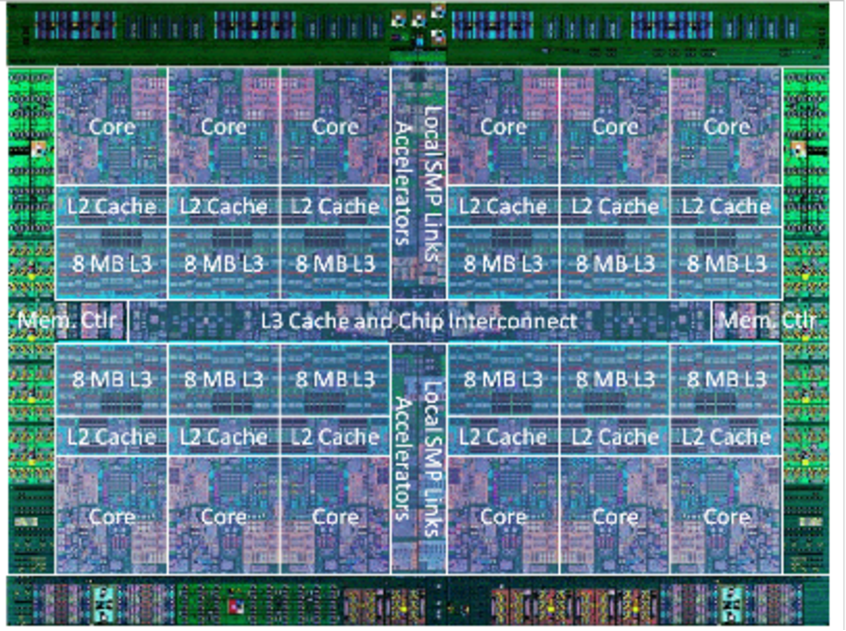
\includegraphics[width=1.0\textwidth]{./Images/P8.pdf}}
%  	\vspace{-0.0pc}
	 \caption{Power8 processor chip.~\cite{IBM_P8}}
 	 \label{fig:p8_1}
    \end{subfigure}
     \centering
    \begin{subfigure}[b]{0.4\textwidth}
         {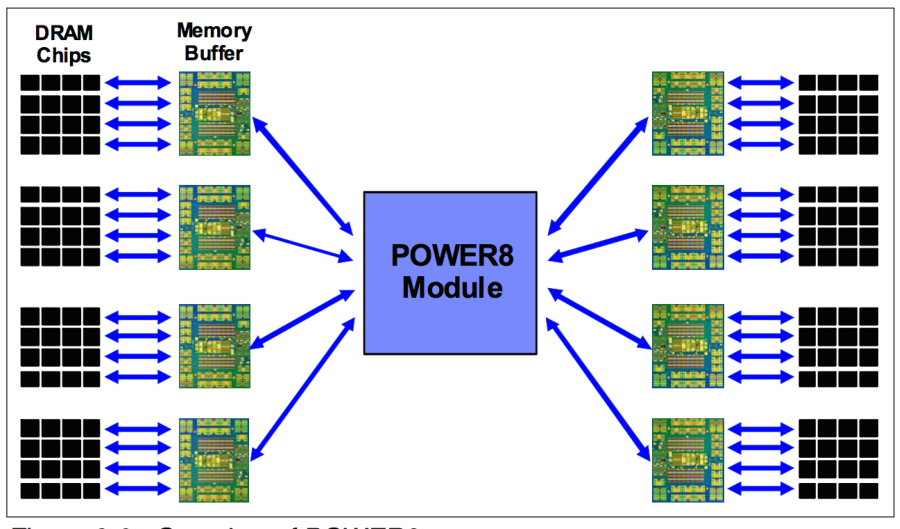
\includegraphics[height=0.7\textwidth]{./Images/P8_memory.pdf}}
  %	\vspace{-0.0pc}
	 \caption{Power8 Memory Access.~\cite{IBM_P8}}
	  \label{fig:p8_2}
    \end{subfigure}
  \caption{POWER8 Overview}\label{fig:POWER8}
\end{figure}
The POWER8 system has a Non-Uniform Cache Architecture (NUCA) Cache Policy, this allows for scalable bandwidth and latency, allowing migration of most used cache lines to the local L2 cache and then to the local L3 cache~\cite{IBM_P8}. This is a big improvement over the POWER7 processor.  Each cache level will have a cost for accessing data locally vs remote.  

%When we run the command  \textit{numactl} the operating system reports the following NUMA nodes on a two socket POWER8 system. 
A NUMA distance is the ratio between the latency of accessing  a remote numa node memory and local memory access. To illustrate this,  when we run the command \textit{numactl} on a two socket POWER8 system, we get the following 
NUMA nodes and distances (see ~\ref{fig:crest}): 

\begin{figure}[h]
  \centering
  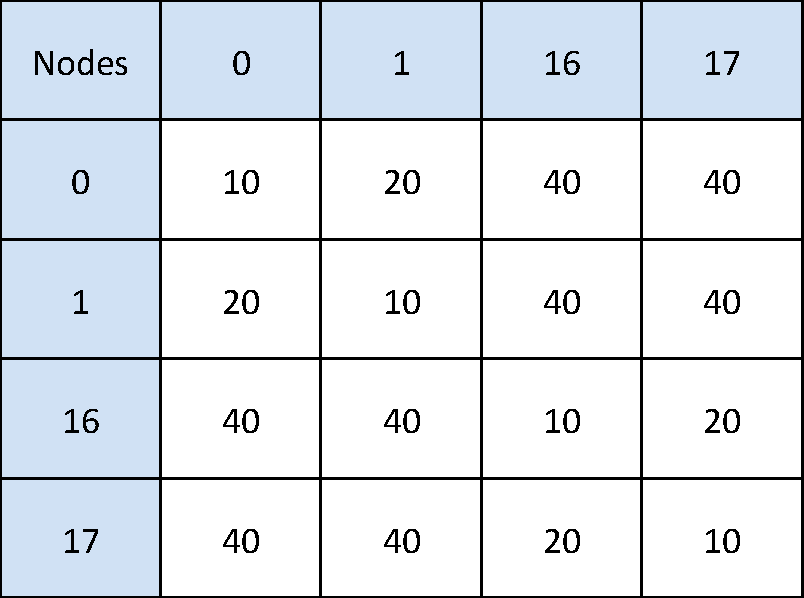
\includegraphics[height=0.3\textwidth]{./Images/crest.pdf}
       \caption{\textit{Numactl} hardware characteristics of a two socket POWER8 system}
       \label{fig:crest}
\end{figure}

%[4/9/16, 12:37:55 PM] Oscar: we just need to expand the text for that table
%[4/9/16, 12:38:07 PM] Oscar: we need to explain why we have these numbers in blue
%[4/9/16, 12:38:25 PM] Oscar: and why we have these many rows and columns
%[4/9/16, 12:38:38 PM] Oscar: and how that related to a dual socket POWER8 system



 